\begin{figure}[htbp]
	\centering
	\newcommand\sfMergeRealImag{0.9}
	\newcommand\gridnode[5]{
		\node (#1) at (#2 + #4 / 2,#3 + #5 / 2) [minimum width=#4cm * \sfMergeRealImag,minimum height=#5cm * \sfMergeRealImag] {};
		\draw[step=0.1] (#2 - 0.001,#3 - 0.001) grid (#2+#4 + 0.001,#3+#5 + 0.001);	
	}
	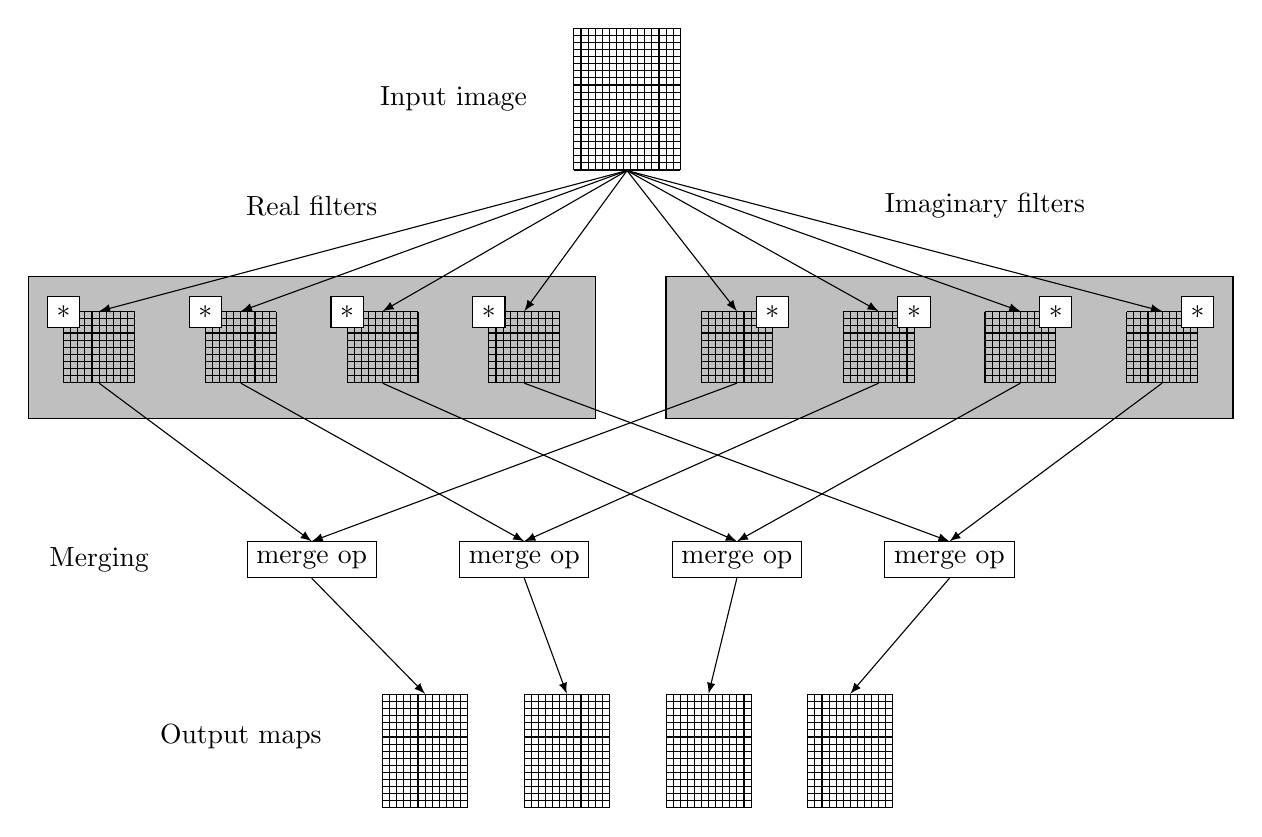
\begin{tikzpicture}[scale=\sfMergeRealImag,every path/.style={>=latex}]
		% draw input image
		\gridnode{inputimage}{7.7}{3}{1.5}{2}
	
		% draw background boxes
		\draw[fill=lightgray] (0,1.5) rectangle (8,-0.5);
		\draw[fill=lightgray] (9,1.5) rectangle (17,-0.5);
	
		% draw real filters
		\foreach \x in {0,...,3}
		{
			\gridnode{r\x}{\x * 2 + 0.5}{0}{1}{1}
			\node at (\x * 2 + .5, 1) [draw,fill=white] {$*$};
			\draw[->] (inputimage.south) to (r\x.north);
		}
		
		% draw imaginary filters
		\foreach \x in {0,...,3}
		{
			\gridnode{i\x}{\x * 2 + 9.5}{0}{1}{1}
			\node at (\x * 2 + 10.5, 1) [draw,fill=white] {$*$};
			\draw[->] (inputimage.south) to (i\x.north);
		}
		
		% draw merge operators
		\foreach \x in {0,...,3}
		{
			\node (m\x) at (\x * 3 + 4,-2.5) [draw,rectangle] {merge op};
			\draw[->] (r\x.south) to (m\x.north);
			\draw[->] (i\x.south) to (m\x.north);
		}
		
		% draw output maps
		\foreach \x in {0,...,3}
		{
			\gridnode{o\x}{\x * 2 + 5}{-6}{1.2}{1.6}
			\draw[->] (m\x.south) to (o\x.north);
		}
		
		% draw text nodes
		\node at (6,4) {Input image};
		\node at (4,2.5) {Real filters};
		\node at (13.5,2.5) {Imaginary filters};
		\node at (1,-2.5) {Merging};
		\node at (3.,-5) {Output maps};
	\end{tikzpicture}
	\caption{Merging the real and the imaginary filters}
	\label{fig:merge_real_imag}
\end{figure}
